\subchapter{Setup BeagleBone Black board}{Objectives: Set up serial
  communication with the development workstation.}

\section{Setting up serial communication with the board}

The Beaglebone serial connector is exported on the 6 pins close to one
of the 48 pins headers. Using your special USB to Serial adapter, connect
the ground wire (blue) to the pin closest to the power supply connector
(let's call it pin 1), and the \code{TX} (red) and \code{RX} (green) wires
to the pins 4 (board \code{RX}) and 5 (board \code{TX}).

You always should make sure that you connect the \code{TX} pin of the cable
to the \code{RX} pin of the board, and vice versa, whatever the board and
cables that you use.

\begin{center}
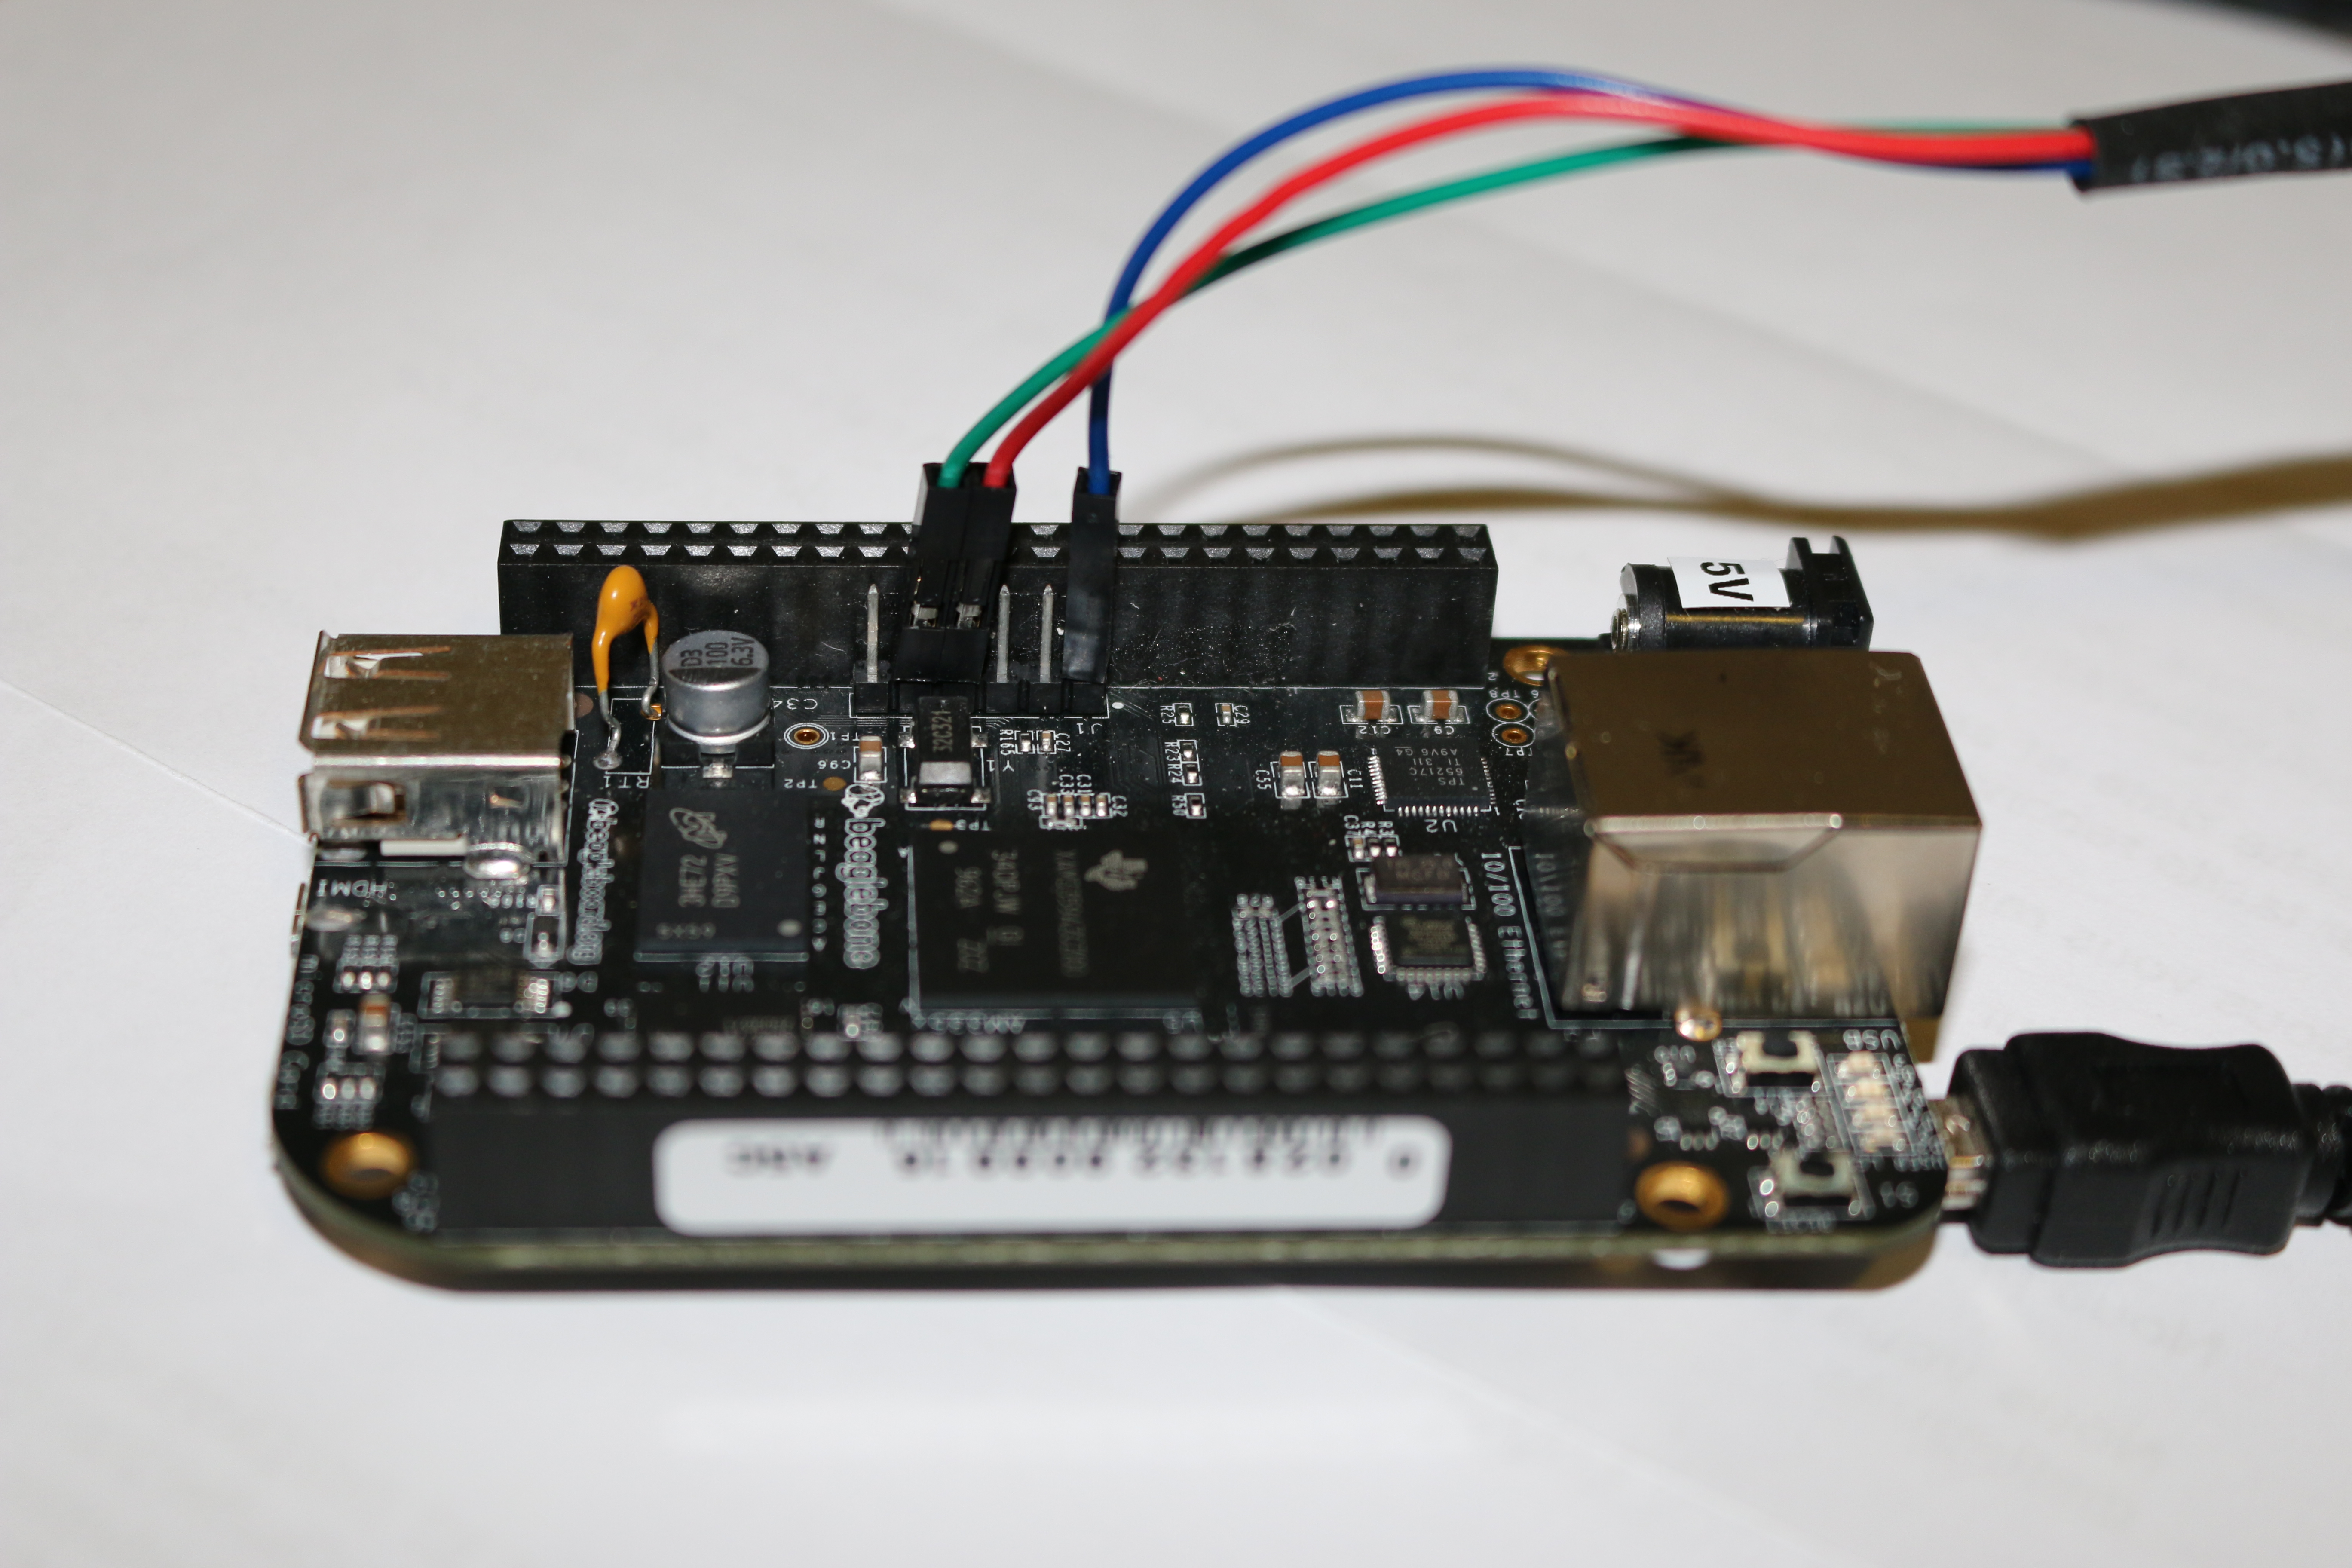
\includegraphics[width=8cm]{labs/setup-bbb-board/beaglebone-black-serial-connection.jpg}
\end{center}

Once the USB to Serial connector is plugged in, a new serial port
should appear: \code{/dev/ttyUSB0}.

You can also see this device appear by looking at the output of
\code{sudo dmesg}.

To communicate with the board through the serial port, install a
serial communication program, such as \code{picocom}:

\bashcmd{$ sudo apt install picocom}

If you run {\tt ls -l \hosttty}, you can also see that only
\code{root} and users belonging to the \code{dialout} group have
read and write access to the serial console. Therefore, you need
to add your user to the \code{dialout} group:

\bashcmd{$ sudo adduser $USER dialout}

{\bf Important}: for the group change to be effective, you have to
reboot your computer (at least on Ubuntu 20.04) and log in again.
A workaround is to run \code{newgrp dialout}, but it is not global.
You have to run it in each terminal.

Run {\tt picocom -b 115200 \hosttty}, to start serial
communication on {\tt \hosttty}, with a baudrate of 115200.
If you wish to exit \code{picocom}, press \code{[Ctrl][a]} followed by
\code{[Ctrl][x]}.

There should be nothing on the serial line so far, as the board is not
powered up yet.

It is now time to power up your board by plugging in the mini-USB
(BeagleBone Black case) cable to your PC.

See what messages you get on the serial line. You should see U-boot
start on the serial line, if there was a valid U-Boot and SPL on the board's eMMC.
